\documentclass{article}
\usepackage[T1]{polski}
\usepackage[utf8]{inputenc}
\usepackage[pdftex]{graphicx}
\usepackage[top=1in, bottom=1in, left=1in, right=1in]{geometry}
\pagestyle{empty} 

\newenvironment{nscenter}
 {\parskip=0pt\par\nopagebreak\centering}
 {\par\noindent\ignorespacesafterend}
 
\begin{document}
  \centering{\textbf{Top Prover}}
  
  \begin{enumerate}
   \item \textbf{Opis aplikacji}\\
TopProver jest stroną zajmującą się organizowaniem konkursów matematycznych. 
Jej nadrzędnym celem jest zapewnienie rozwiązań skomplikowanych problemów, 
które muszę być rozwiązane w krótkich przedziałach czasowych, jak również szerzenie wiedzy z zakresu
nauk matematycznych i rozwijanie zdolności dowodzenia i rozwiązywania problemów 
powiązanych z powyższą dziedziną.

Aby realizacja tego zadania była możliwa organizowane są konkursy w których mogą brać wszyscy
zainteresowani matematyką użytkownicy ww. serwisu. Celem każdego "meczu" jest rozwiązanie zadania 
zaproponowanego przez zleceniodawcę, któremu zależało na szybkim jego rozwiązaniu. 

Motywacją dla osób chcących spróbować swoich sił w tej rywalizaji są nagrody pieniężne fundowane przez 
autorów zadań dla autorów rozwiązań wygrywających konkurs.

Aby umożliwić zleceniodawcy otrzymanie porządanych rezultatów związanych z konkursem, strona umożliwia mu wybór,
czy jako wynik konkursu chce otrzymać:
\begin{itemize}
 \item najlepsze rozwiązanie (najwyżej ocenione przez sprawdzających)
 \item określoną liczbę rozwiązań najlepszych (na przykład by otrzymać pulę różnych możliwych rozwiązań, lub samodzielny wybór najlepszego)
 \item najszybciej wyłonione poprawne rozwiązanie
\end{itemize}

W ten sposób TopProver z jednej strony umożliwia uzyskanie dobrego rozwiązania danego zagadnienia w krótkim czasie,
jak i motywowanie społeczności matematyków do nieustannego próbowania swoich sił w kolejnych zawodach.\\
\hrulefill

\begin{nscenter}
Punkty i hierarchia użytkowników
\end{nscenter}
\newline
Użytkownicy naszego serwisu rozwiązujący zadania będą nagradzani zarówno określonymi przez zleceniodawców gratyfikacjami finansowymi,
jak i punktami przydzielanymi przez sprawdzających nadesłane rozwiązania za poprawność, przejrzystość, dokładnośc i prostotę.
Po zdobyciu określonej ilości punktów użytkownicy mogą być awansowani do rangi sprawdzających, co wiąże się z dodatkowymi uprawnieniami w serwisie.
Sprawdzający którzy zweryfikowali poprawnie najwięcej rozwiązań nagradzani są okresowo wynagrodzeniem przyznawanym przez serwis,
wypłacanym ze środków uzyskanych za prowadzenie konkursów od autorów problemów.

Większa liczba punktów umożliwi nie tylko komentowanie, a z czasem nawet weryfikacje prac innych matematyków,
ale również zapewni dostęp do okresowych konkursów dla bardziej zaawansowanych użytkowników.

Ww. zawody będą się wyróżniać w stosunku do standardowych zawodów tym,
że problemy w nich zaprezentowane będą nieco trudniejsze a nagrody oferowane za ich rozwiązanie znacząco wyższe od tych,
które można spotkać w dostępnym dla wszystkich zalogowanych osób module konkursowym.\\
\hrulefill
\begin{nscenter}
Moduł edukacyjny
\end{nscenter}
\newline
Dla użytkowników chcących przejrzeć wcześniej rozwiązane problemy zostanie otworzony moduł edukacyjny.
Będzie on biblioteką zawierającą wszystkie pytania pochodzące z modułu konkursowego uzupełnione o pare najlepszych odpowiedzi. 

Dostęp do tej części serwisu będzie nieograniczony. Dzięki temu każdy będzie mieć kontakt z realnymi problemami nad jakimi pracują matematycy.

\newpage
   \item \textbf{Model działania aplikacji}
    \begin{enumerate}
     \item Podstawowy schemat (niezalogowany użytkownik)
      \begin{itemize}
       \item Rejestracja konta
       \begin{itemize}
        \item login
        \item hasło
        \item tagi (określające zainteresowania użytkownika)
        \item mail oraz opcje subskrypcji
       \end{itemize}
       \item Logowanie
       \begin{itemize}
        \item login
        \item hasło
       \end{itemize}

      \end{itemize}
     \item Podstawowy schemat (zalogowany użytkownik)
     \begin{itemize}
      \item Zmiana ustawień konta (hasła, maila, tagów, opcji dot. subskrypcji)
      \item Składanie zamówienia
      \item Przeglądanie listy dostępnych konkursów\\
	    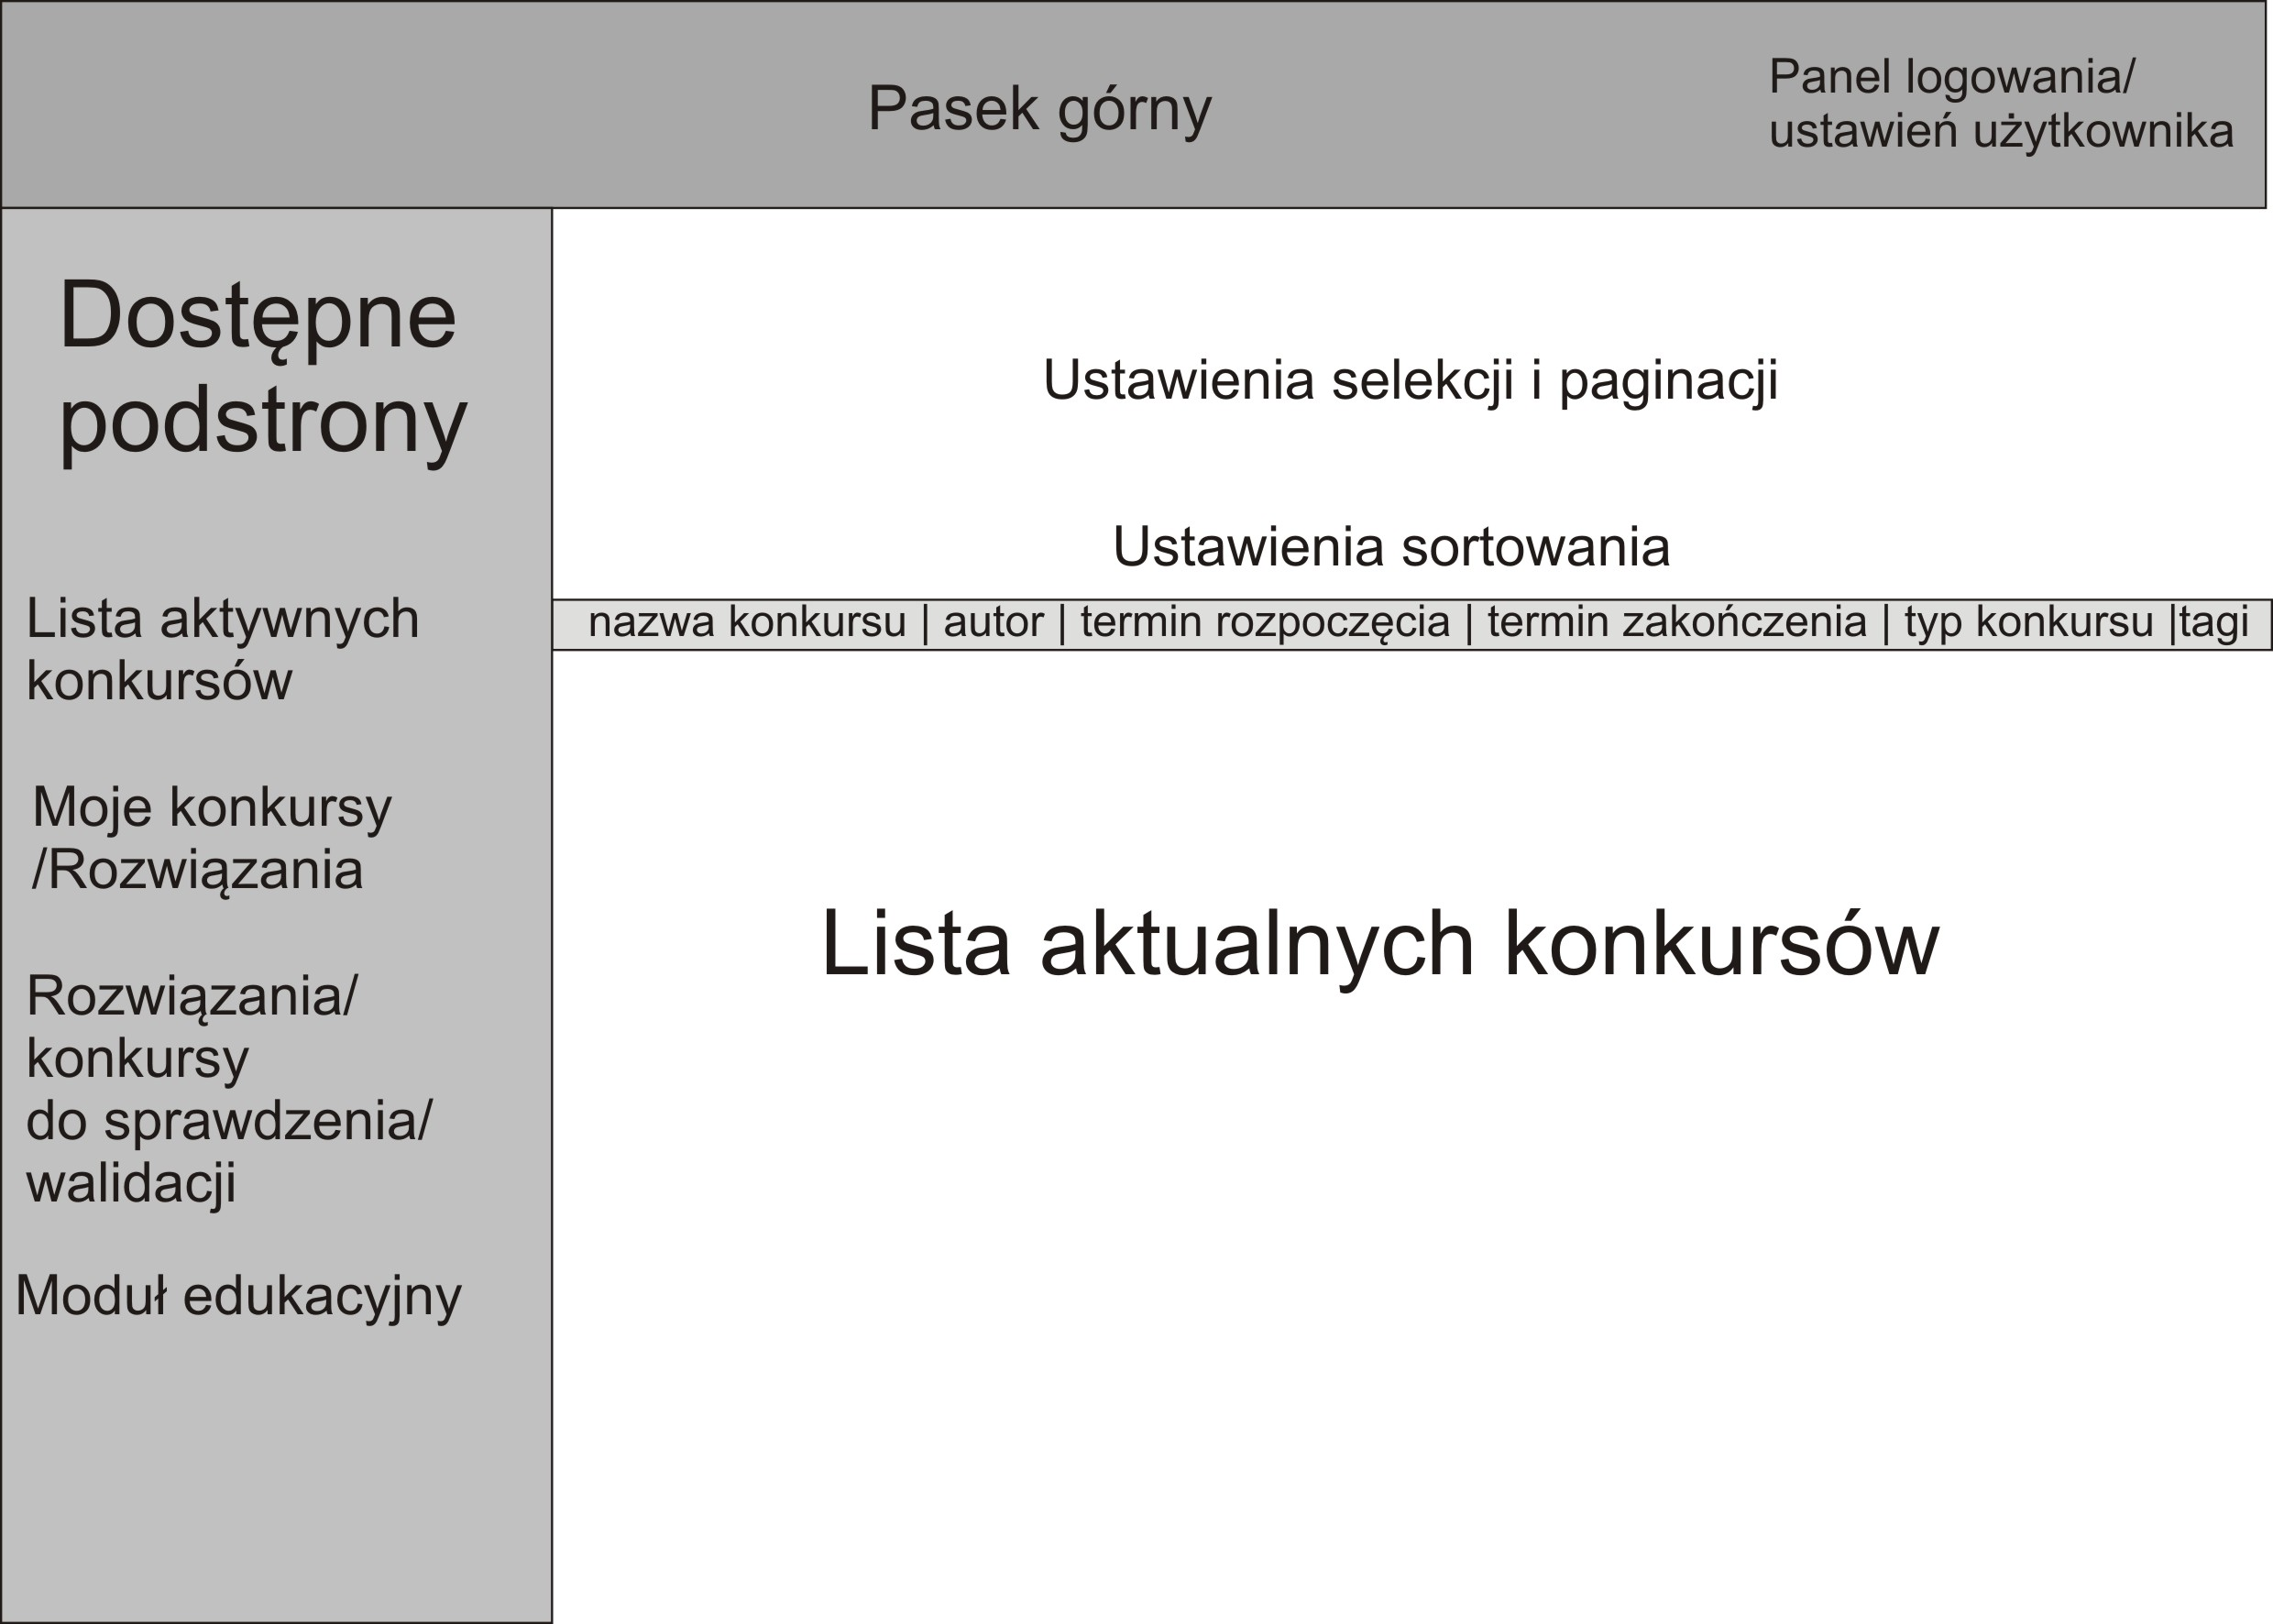
\includegraphics[scale=0.5]{IO_rysunki.jpg}
      \begin{itemize}
       \item istnieje możliwośc zadeklarowania checi zostania sprawdzającym dla jednego z wątków
      \end{itemize}
      \item Przeglądanie pozycji w obrębie modułu edukacyjnego

     \end{itemize}
     \newpage
     \item Proces realizacji zamówienia
     \begin{itemize}
      \item Składanie zamówienia\\
	    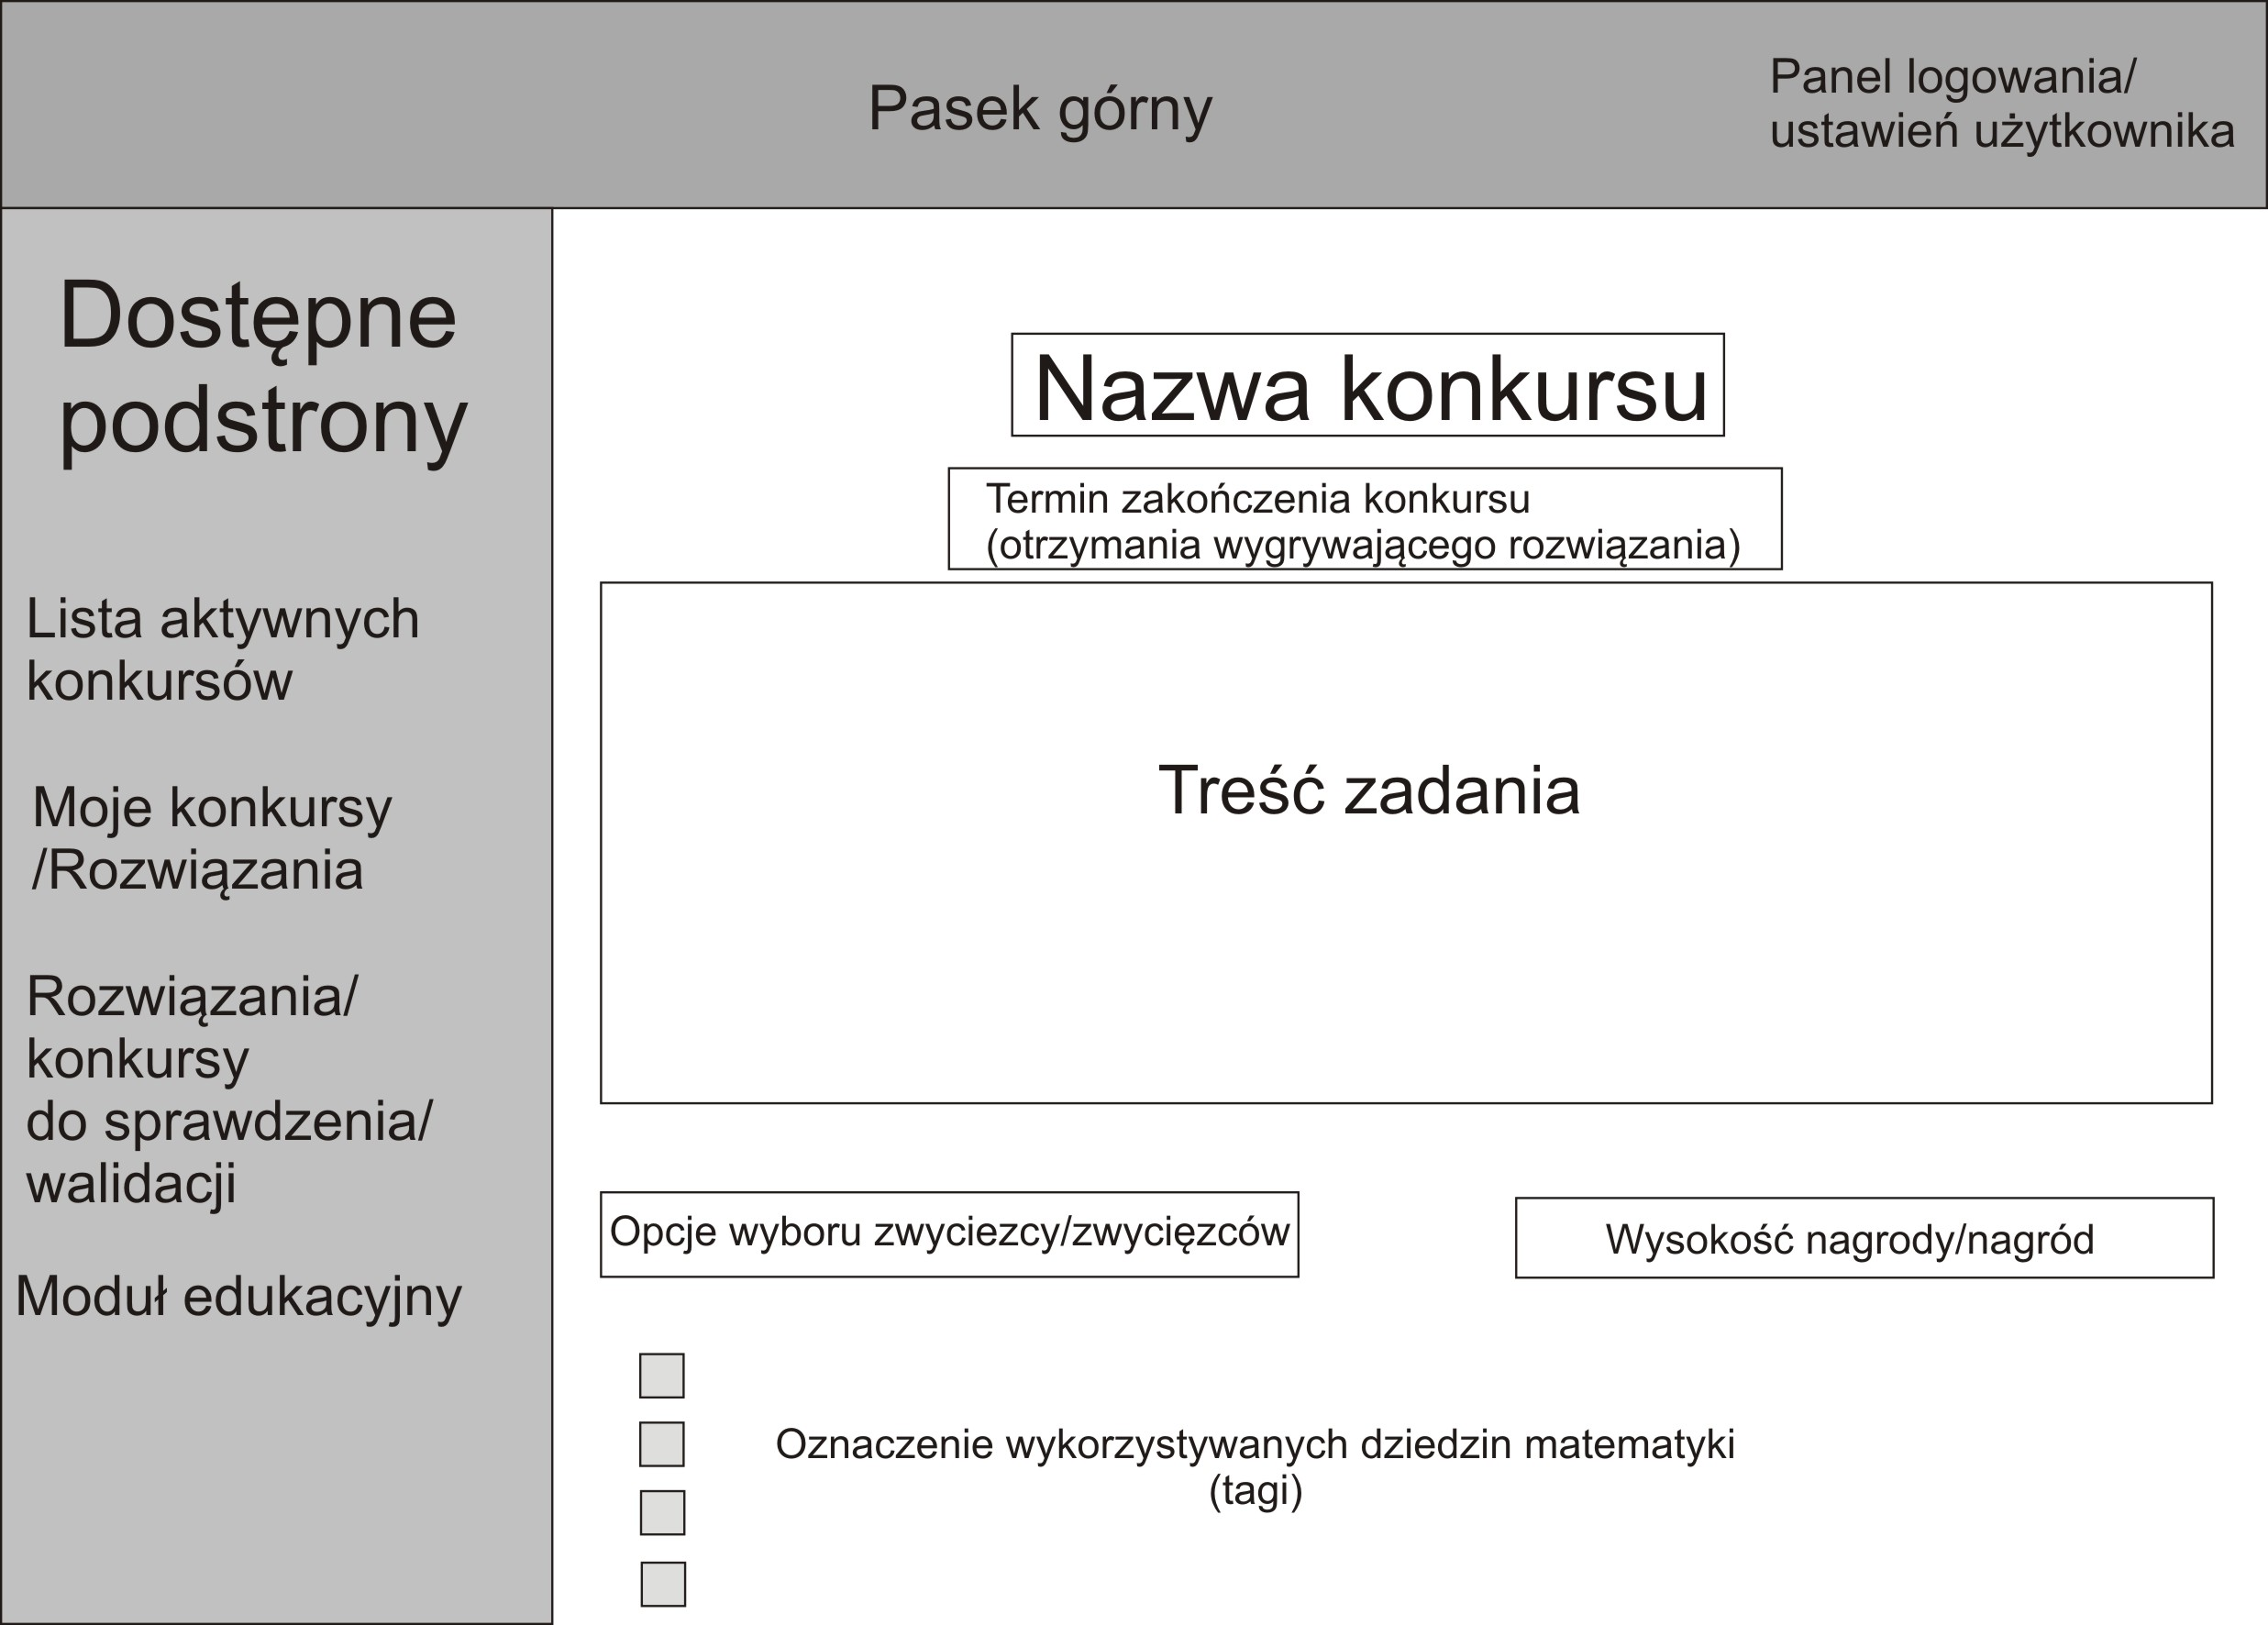
\includegraphics[scale=0.5]{IO_rysunki3.jpg}  
      \item Wysyłanie rozwiązań
      \item Sprawdzanie rozwiązań
	\begin{itemize}
	 \item Dla każdego zagadnienia istnieje pula osób, które deklaruja chęć sprawdzania prac
	 \item Dla danej pracy losuje sie (przy uwzględnieniu tagów) określoną liczbę osób, które będą ją weryfikować
	 \item Sprawdzona praca (wraz z komentarzami i punktami) jest przesyłana do jej autora
	 \begin{itemize}
	  \item autor zadania może trzy razy wysłać poprawiona wersję po odczekaniu wyznaczonego terminu - taka decyzja spowoduje wykasowanie wczesniejszej wersji.
	  Ww. korekta pojawia się w systemie jako zupełnie nowa praca.
	 \end{itemize}

	 \item Pojedyncza osoba może albo przesłać dla danego zadania rozwiązanie albo być sprawdzającym (nie może pełnić tych 2. funkcji jednocześnie)
	 \item Jeśli liczba przesłanych prac jest niewielka, to mogą być one sprawdzane wiecej razy (gdy jest mało prac, to każda praca moze być sprawdzana 2-3 krotnie przez 2-3 różne osob)
	 \item Każdemu rozwiązaniu osoby sprawdzające przyznają punkty (np. za elegancje, dokładność, przejrzystość, prostotę)
	\end{itemize}
      \item Weryfikacje wybranych sprawdzeń
      \begin{itemize}
	 \item Losowo wybrane oceny prac są dodatkowo sprawdzane, aby zminimalizować ilość błędnych ocen.
	 \item Weryfikowane jest rozwiązanie/rozwiązania wybrane jako wygrywające.
	 \item Dodatkowo istnieje możliwość weryfikacji w przypadku zgłoszenia przez autora rozwiązania niepoprawnej/niesprawiedliwej oceny.
	 \item Wynikiem weryfikacji jest przyznanie punktów (być może ujemnych) sprawdzającemu, oraz ewentualna zmiana oceny rozwiązania.
      \end{itemize}
      
      \item Przesyłanie wyniku zleceniodawcy
	\begin{itemize}
	 \item Przesyłany jest jeden lub kilka najlepszych projektów (w zależności od preferencji określonych przez zleceniodawce w trakcie składania zamówienia)
	 \item Zleceniodawca jest zabowiązany informować przy każdym użyciu wyników powstałych w trakcie realizacji zlecenia o tym, kto jest autorem tego rozwiązania,
	 jak również o tym, że ww. rozwiązanie powstało dzięki współpracy z serwisem TopProver.
	 \item Autor najlepszego rozwiązania otrzymuje dodatkowe punkty określające jego pozycję w hierarchii serwisu,
	 jak również gratyfikację finansową o wartości zależnej od kwoty przeznaczonej przez zleceniodawcę przy składaniu zamówienia
	\end{itemize}

     \end{itemize}
    \newpage
    \item Przebieg konkursu
    \begin{itemize}
     \item Po wysłaniu zamówienia przez jego autora jest ono analizowane przez użytkownika o wysokim statusie (administratora, moderatora, wysokopunktowanego sprawdzającego)
     pod kątem poprawności sformułowania, wystarczalności czasu, wystarczającej wysokości nagrody.
     \item Po dopuszczeniu konkurs pojawia się na liście aktywnych konkursów, wysyłane są ewentualne maile (lub następuje dopisanie do maila w wypadku wysyłania okresowego).
     \item Użytkownicy mogą wysłać rozwiązanie albo zgłosić się do jego sprawdzania. Można również czytać aktualne komentarze i dopisywać własne\\
	  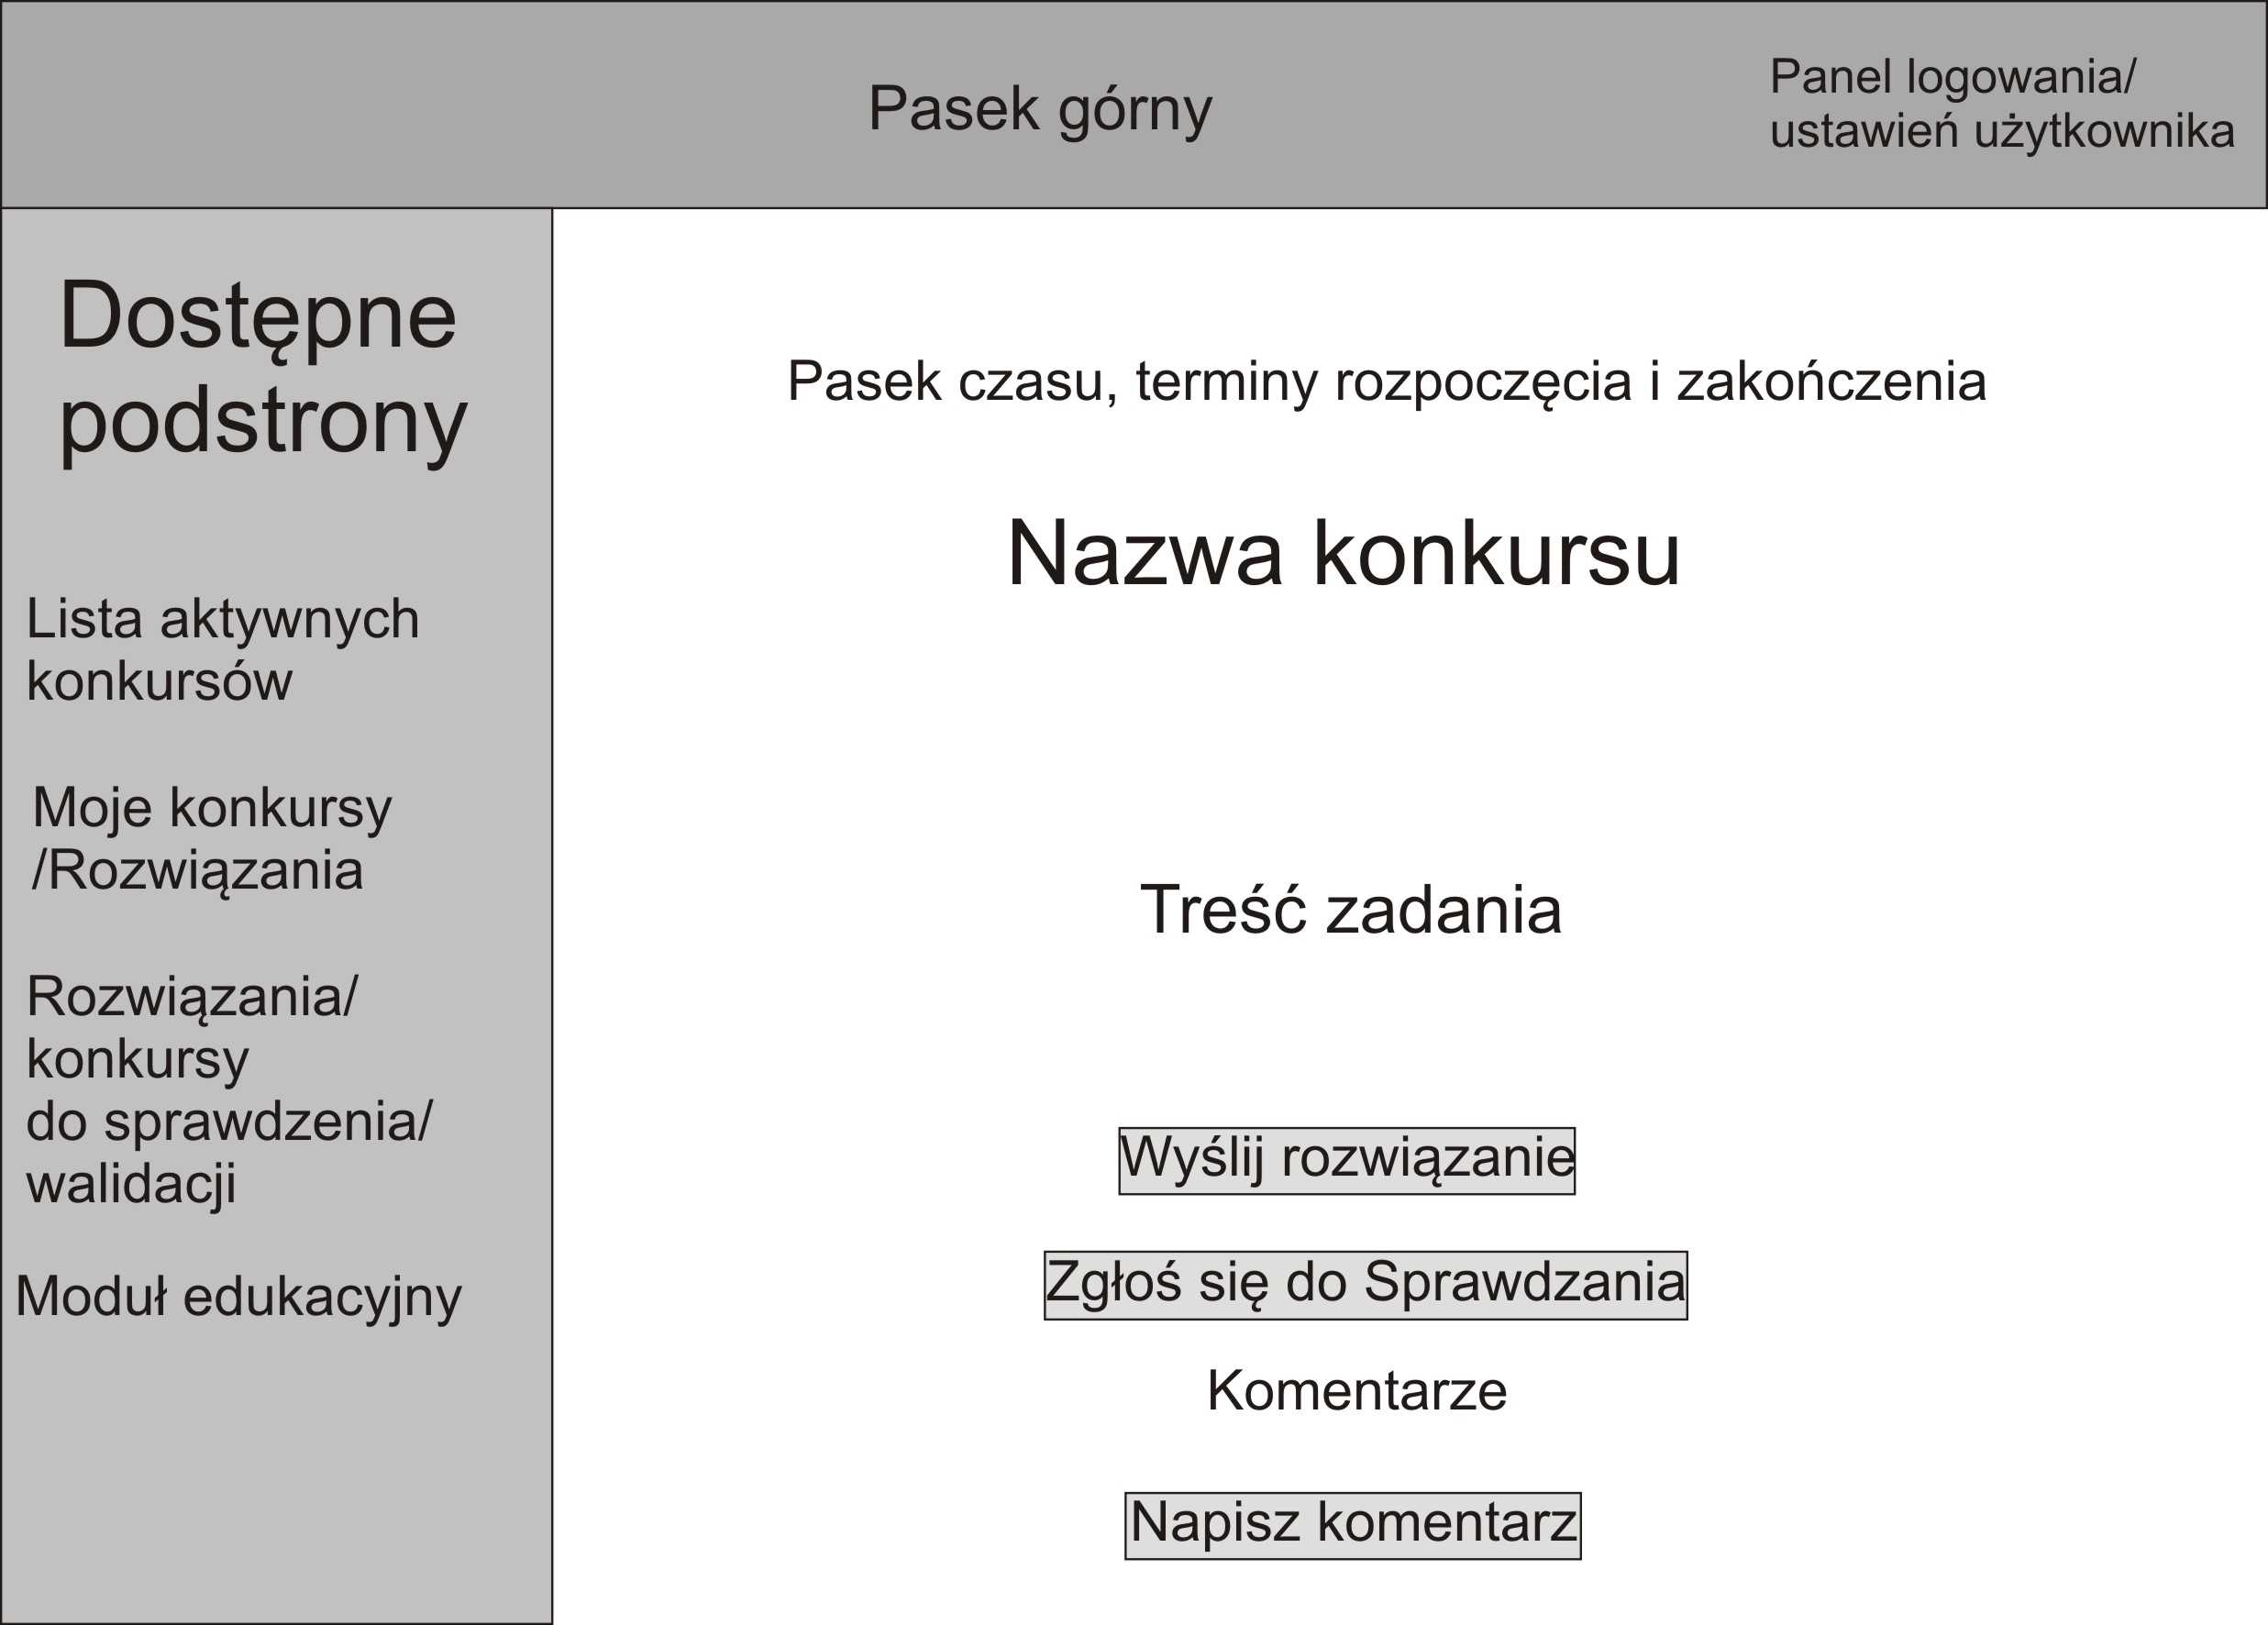
\includegraphics[scale=0.5]{IO_rysunki2.jpg}      
     \item Po pojawieniu się rozwiązania w systemie losowany jest sprawdzający spośród tych których tagi zgadzają się w największym stopniu z określonymi w rozwiązaniu
     (jeżeli takich sprawdzających jest zbyt mało, to zasady porównywania tagów stają się mniej restrykcyjne, jeżeli to nie pomaga, to rozwiązanie czeka na ich pojawienie się).
     \item Sprawdzający ma określony czas na sprawdzenie pracy, wpp. jest ona mu odbierana
     (żeby uniknąć rozdawaniu prac osobom, które nie chcą przez pewien czas ich otrzymywać dostepna jest opcja czasowego wyłączenia ze sprawdzania).
     \item Autor rozwiązania po upływie określonego czasu może wysłać poprawkę do rozwiązania. Może on też zgłosić odwołanie do źłej jego zdaniem oceny rozwiązania
     (podając wyczerpującą argumentację).
     \item Wysyłanie rozwiązań zostaje zablokowane w określonym czasie przed datą określoną przez autora zadania. Czas ten jest wykorzystywany na zakończenie sprawdzania 
     i wybór najlepszego z pośród pozytywnie ocenionych rozwiązań.
     \item Autor zadania otrzymuje nagrodzone rozwiązanie/rozwiązania, rozesłane zostają maile informujące i nagrody.
    \end{itemize}
    \newpage
    \item Dodatkowe uwagi
    \begin{itemize}
     \item każdy użytkownik zdobywa punkty rankingowe podczas procesu sprawdzania prac
     \item użytkownicy o wyższym rankingu mogą przyznawać punkty innym użytkownikom za przydatne komentarze do prac

     \item użytkownicy serwisu którzy oznaczyli to w ustawieniach konta otrzymują czas maile z informacjami o nowych problemach,
     które pojawiły się w serwisie i powinny go zainteresować (porównywane są tagi,
     jakie użytkownik określił wcześniej jako interesujące z tagami przypisanymi do konkretnych problemów),
     a także o zmianach w konkursach, w których użytkownik bierze aktywny udział.\newline
     Istnieją 4 mozliwe ustawienia subskrypcji:
      \begin{enumerate}
       \item Brak otrzymywania maili od serwisu.
       \item Otrzymywane maile wyłącznie dotyczące konkursów, w których użytkownik bierze aktywny udział
       (zakończenie konkursu, informacja o wyłonieniu jako laureata, informacja o dokonanej ocenie wysłanego rozwiązania,
       informacja dla sprawdzającego o nowej pracy przydzielonej do sprawdzenia).
       \item Otrzymywanie maili o konkursach w których użytkownik bierze udział, oraz o pojawieniu się nowych konkursów, zgodnych z zainteresowaniami.
       \item Otrzymywanie maili o konkursach w których użytkownik bierze udział, oraz o pojawieniu się nowych konkursów.     
      \end{enumerate}
      \item mechanizm działania tagów (używany np.: przy rozsyłaniu maili, wybieraniu sprawdzających)
	\begin{itemize}
	 \item system nie szuka jednostek (osób, treści) które będą charakteryzowały się idealnym dopasowaniem do tagów wg. ktorych ich przeszukujemy a jedynie stara się je maksymalizować
	 \item oznacza to, że w skrajnym przypadku daną pracę będzie musiała sprawdzać osoba, która nie zadeklarowała checi zajmowania się daną tematyką
	 \item taka decyzje usprawiedliwia fakt, że wszyscy sprawdzajacy będą musieli dysponować pewną wiedzą z zakresu matematyki wyższej
	\end{itemize}


    \end{itemize}

    
    \end{enumerate}

   \item \textbf{Podstawowe założenia}
    \begin{itemize}
     \item Strona dysponuje kapitałem początkowym potrzebnym do rozpoczęcia działalności
     \item Strona dysponuje pewną startową pulą osób odpowiedzialnych za sprawdzanie prac
      \begin{itemize}
       \item grupa wyżej wymienionych osób będzie wyłoniona w procesie rekrutacji spośród studentów II stopnia / doktorantów matematyki
      \end{itemize}

    \end{itemize}

  \end{enumerate}


\end{document}